\documentclass[14pt]{extarticle}

% -----------------------------
% General (big, readable) whitepaper styling
% -----------------------------
\usepackage[T1]{fontenc}
\usepackage{lmodern}
\usepackage[margin=1in]{geometry}
\usepackage[protrusion=true,expansion=true]{microtype}
\usepackage{setspace}
\usepackage{graphicx}
\usepackage{xcolor}
\usepackage{booktabs}
\usepackage{array}
\usepackage{amsmath,amssymb}
\usepackage{enumitem}
\usepackage{url}
\usepackage{hyperref}
\usepackage{cleveref}
\usepackage{listings}
\usepackage{fancyhdr}
\usepackage{titlesec}

% Better page breaks with larger font
\usepackage{nowidow}

% Simple diagrams
\usepackage{tikz}
\usetikzlibrary{arrows.meta,positioning,shapes.geometric}

% Callout boxes
\usepackage{tcolorbox}
\tcbset{colback=black!2,colframe=black!25,arc=2pt,boxrule=0.6pt,left=6pt,right=6pt,top=6pt,bottom=6pt}

\hypersetup{hidelinks}

% Slightly more spacious, ``general paper'' feel
\setstretch{1.15}
\setlist[itemize]{leftmargin=*,topsep=0.3em,itemsep=0.2em}
\setlist[enumerate]{leftmargin=*,topsep=0.3em,itemsep=0.2em}

\titleformat{\section}{\Large\bfseries}{\thesection}{0.6em}{}
\titleformat{\subsection}{\large\bfseries}{\thesubsection}{0.6em}{}

% -----------------------------
% Header / footer
% -----------------------------
\pagestyle{fancy}
\fancyhf{}
\lhead{ExtremeSniffer Whitepaper}
\rhead{\thepage}
\renewcommand{\headrulewidth}{0.4pt}

% -----------------------------
% Listings setup (C++)
% -----------------------------
\lstdefinelanguage{ModernC++}{
  language=[11]C++,
  morekeywords={constexpr,noexcept,nullptr,thread,mutex,unique_lock,lock_guard,condition_variable,atomic,unordered_map,unordered_set,chrono},
}

\lstset{
  language=ModernC++,
  basicstyle=\ttfamily\small,
  keywordstyle=\bfseries\color{black},
  commentstyle=\itshape\color{gray!70!black},
  stringstyle=\color{black},
  columns=fullflexible,
  keepspaces=true,
  breaklines=true,
  frame=single,
  rulecolor=\color{black!20},
  numbers=left,
  numberstyle=\scriptsize\color{black!55},
  xleftmargin=2.0em,
  framexleftmargin=1.8em,
  aboveskip=0.75em,
  belowskip=0.75em,
}

% -----------------------------
% Document metadata
% -----------------------------
\title{\textbf{ExtremeSniffer}\\\vspace{0.25em}
\large A Practical Whitepaper on a Multithreaded C++ Network Capture, Inspection, and Anomaly Alerting Tool}

\author{\textbf{Project Team}\\
\normalsize General Documentation}

\date{\normalsize \today}

\begin{document}

% -----------------------------
% Title page
% -----------------------------
\begin{titlepage}
  \centering
  \vspace*{1.0cm}

  {\Huge\bfseries ExtremeSniffer\par}
  \vspace{0.35cm}
  {\Large\bfseries Practical Whitepaper\par}
  \vspace{0.8cm}

  \begin{minipage}{0.92\textwidth}
    \large
    This document describes the imported C++ network security application in a clear, operator-focused way. It is intended for developers, students, and security practitioners who want to understand what the tool does, how it is built, how to run it, and what to expect in real environments.
  \end{minipage}

  \vspace{1.0cm}

  \IfFileExists{visual/banner.jpg}{%
    \includegraphics[width=0.92\textwidth]{visual/banner.jpg}\par
  }{%
  }

  \vfill

  {\large Version: 1.1\par}
  {\large Date: \today\par}
\end{titlepage}

\tableofcontents
\vspace{0.6cm}

\section{Executive Summary}
ExtremeSniffer is a practical C++ network security tool that captures live traffic, inspects packets for actionable protocol fields, and generates structured alerts when it observes behaviors that commonly correlate with reconnaissance or denial-of-service activity.

It uses \texttt{libpcap} for packet capture and BPF filtering, and can enrich public IP addresses with GeoIP metadata using \texttt{libmaxminddb} and the GeoLite2 City database.\cite{libpcap,bpf,maxminddb,geolite2}

\begin{tcolorbox}[title=At a glance]
\begin{itemize}
  \item \textbf{Primary value:} fast visibility + explainable detections you can tune.
  \item \textbf{Output:} JSON alerts that can be redirected to a file, forwarded, or ingested by a SIEM.
  \item \textbf{Core detections:} port scanning, connection flooding, packet flooding.
  \item \textbf{Best fit:} labs, demos, lightweight host sensors, and prototyping.
  \item \textbf{Not a replacement for:} full IDS/NDR platforms (e.g., Zeek/Suricata).\cite{zeek,suricata}
\end{itemize}
\end{tcolorbox}

\subsection{What You Get Out of It}
\begin{itemize}
  \item A clear, inspectable stream of security-relevant network events.
  \item A baseline detection layer that can catch ``loud'' scanning and flood activity.
  \item A codebase you can extend (parsers, counters, new alert types) without adopting a full IDS framework.
\end{itemize}

\subsection{Scope and Assumptions}
This tool focuses on packet capture + lightweight behavior heuristics. It does \emph{not} attempt full protocol normalization, TCP stream reassembly, or signature rulesets. In environments where traffic is heavily encrypted, the tool primarily operates on L3/L4 metadata (IPs, ports, rates).

\section{What This Tool Does (In Plain Terms)}
Think of ExtremeSniffer as a real-time ``network microscope'' with an alarm.

\subsection{Runtime Workflow}
\begin{enumerate}
  \item \textbf{Listen:} open a capture handle on a network interface.
  \item \textbf{Filter:} optionally apply a BPF filter to reduce noise.\cite{bpf}
  \item \textbf{Capture:} receive packets in real time.
  \item \textbf{Parse:} extract L2/L3/L4 fields; attempt HTTP/DNS hints when visible.
  \item \textbf{Score:} update per-source counters/sets and compare against thresholds.
  \item \textbf{Alert:} output JSON events with context (and GeoIP when available).
\end{enumerate}

\subsection{What It \emph{Does Not} Do}
\begin{itemize}
  \item It does not ``decrypt'' TLS/HTTPS.
  \item It does not provide a full rules engine (signatures) like a traditional IDS.
  \item It does not guarantee lossless capture on very high-throughput links.
\end{itemize}

\section{Intended Audience and Use Cases}
\subsection{Audience}
\begin{itemize}
  \item Developers who want a readable reference implementation for \texttt{libpcap}.\cite{libpcap}
  \item Students learning network protocols, packet formats, and defensive telemetry.
  \item Security engineers who want a small tool for lab validation, demos, and quick investigations.
\end{itemize}

\subsection{Common Use Cases}
\begin{itemize}
  \item Detect obvious scanning in a training lab.
  \item Verify that firewall/rate-limit changes reduce scanning or flooding symptoms.
  \item Enrich alerts with GeoIP context for reporting (where legally appropriate).
  \item Prototype new detections before porting ideas to a larger platform.
\end{itemize}

\subsection{Where It Fits in a Security Stack}
\begin{tcolorbox}[title=Positioning]
Use ExtremeSniffer as a \textbf{sensor} and \textbf{event generator}. If you later need deep protocol analytics, signature rules, or enterprise-scale management, pair it with (or migrate to) Zeek/Suricata/Snort-style tooling.\cite{zeek,suricata,snort}
\end{tcolorbox}

\section{Key Features (Enhanced)}
\begin{itemize}
  \item \textbf{Real-time capture} using \texttt{libpcap}.\cite{libpcap}
  \item \textbf{BPF traffic filtering} for precision collection and performance.\cite{bpf}
  \item \textbf{Multithreaded analysis pipeline} (capture thread + worker threads).
  \item \textbf{DPI-style parsing} to extract operator-useful fields (IP/ports + opportunistic HTTP/DNS hints).
  \item \textbf{Explainable heuristic detections} with tunable thresholds and low operational complexity.
  \item \textbf{GeoIP enrichment} via MaxMind DB + GeoLite2.\cite{maxminddb,geolite2}
  \item \textbf{Operator-friendly JSON output} for easy downstream integration.
\end{itemize}

\section{Project Layout (Imported)}
\begin{itemize}
  \item \texttt{ExtremeSniffer.cpp}: primary implementation.
  \item \texttt{NetworkSniffer.cpp}: simpler baseline sniffer.
  \item \texttt{CybersecurityAnalysis.md}: deeper security discussion.
  \item \texttt{visual/}: documentation images.
\end{itemize}

\section{Architecture (How the Tool Is Built)}
\subsection{High-Level Pipeline}
\begin{enumerate}
  \item \textbf{Capture:} pull packets from the OS capture path (fast path).
  \item \textbf{Queue:} push packet metadata into a bounded buffer.
  \item \textbf{Parse:} decode L2/L3/L4 headers, then attempt L7 parsing.
  \item \textbf{Aggregate:} update in-memory per-source state (counters/sets).
  \item \textbf{Detect:} evaluate thresholds for scan/flood behaviors.
  \item \textbf{Alert:} emit JSON with context and (optionally) GeoIP.
\end{enumerate}

\subsection{Architecture Diagram}
\begin{center}
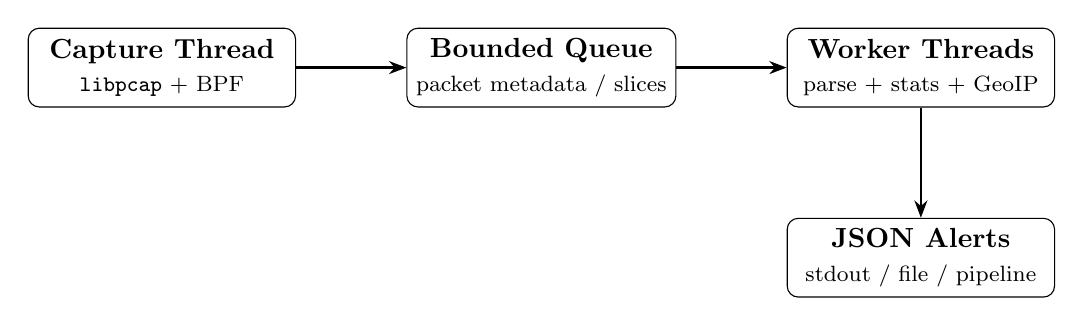
\begin{tikzpicture}[
  node distance=14mm,
  box/.style={draw,rounded corners,align=center,minimum width=0.28\textwidth,minimum height=10mm},
  arr/.style={-{Stealth[length=2.2mm]},thick}
]
\node[box] (cap) {\textbf{Capture Thread}\\\footnotesize \texttt{libpcap} + BPF};
\node[box,right=of cap] (q) {\textbf{Bounded Queue}\\\footnotesize packet metadata / slices};
\node[box,right=of q] (wrk) {\textbf{Worker Threads}\\\footnotesize parse + stats + GeoIP};
\node[box,below=of wrk] (out) {\textbf{JSON Alerts}\\\footnotesize stdout / file / pipeline};

\draw[arr] (cap) -- (q);
\draw[arr] (q) -- (wrk);
\draw[arr] (wrk) -- (out);
\end{tikzpicture}
\end{center}

\subsection{Why Multithreading Matters}
If analysis blocks capture, packets can drop. Separating capture (fast path) from analysis (slow path) helps keep the tool responsive under bursty traffic. The trade-off is synchronization complexity and memory overhead.

\section{Deep Packet Inspection (What We Extract)}
\subsection{Network and Transport Fields}
\begin{itemize}
  \item source/destination IP
  \item source/destination port
  \item protocol (TCP/UDP)
  \item basic sizes/timestamps
\end{itemize}

\subsection{Application Hints (When Visible)}
When payload is in cleartext and recognizable:
\begin{itemize}
  \item \textbf{HTTP:} request method (GET/POST) and user-agent strings.
  \item \textbf{DNS:} query names and record types.
\end{itemize}

\begin{tcolorbox}[title=Reality check: encryption]
In modern networks, much of HTTP is HTTPS and many DNS deployments use DoH/DoT. In those cases, the tool still provides strong L3/L4 metadata (IPs/ports/rates), but it will not reliably extract application-layer fields.
\end{tcolorbox}

\section{Detection Logic (Heuristics)}
These detections are intentionally simple and explainable.

\subsection{Port Scan Indicator}
A typical scan pattern involves one source contacting many distinct destination ports. The tool tracks distinct destination ports per source and triggers when it crosses a threshold.

\subsection{Connection Flood Indicator}
The tool tracks distinct destination endpoints (\texttt{dstIP:dstPort}) contacted by a single source. This catches aggressive probing and some denial-of-service patterns.

\subsection{Packet Flood Indicator}
The tool tracks packet rate/volume per source over a window and alerts when the count is unusually high.

\subsection{Tuning Guidance (Practical)}
\begin{itemize}
  \item Tune thresholds per subnet role (clients vs servers) and per time-of-day.
  \item Add allowlists for known scanners (e.g., vulnerability tools in a controlled lab).
  \item Prefer time-windowed counters with eviction to prevent state growth.
\end{itemize}

\section{GeoIP Enrichment}
GeoIP adds location context to alerts (city/country) by reading a local database file. Lookups can fail for private ranges, missing records, or absent database files.

\section{Build and Run (Operator Notes)}
\subsection{Prerequisites}
\begin{itemize}
  \item C++ compiler (e.g., \texttt{g++})
  \item \texttt{libpcap-dev}\cite{libpcap}
  \item \texttt{libmaxminddb-dev}\cite{maxminddb}
  \item GeoLite2 City database file (e.g., \texttt{GeoLite2-City.mmdb})\cite{geolite2}
\end{itemize}

\subsection{Build}
\begin{lstlisting}[caption={Example build command.},label={lst:build}]
g++ ExtremeSniffer.cpp -o ExtremeSniffer -lpcap -pthread -lmaxminddb
\end{lstlisting}

\subsection{Run}
Packet capture often requires elevated privileges.
\begin{lstlisting}[caption={Example run command.},label={lst:run}]
sudo ./ExtremeSniffer
\end{lstlisting}

\section{Deployment Patterns}
\subsection{Laptop / Lab Host}
Good for learning, demonstrations, and quick checks. Expect more noise (browser updates, background services).

\subsection{Server / Jump Box}
Useful for monitoring east--west traffic on a host and catching obvious floods/scans. Prefer least-privilege capture.

\subsection{SPAN / Mirror Port Sensor (Conceptual)}
Possible in a lab, but high-throughput environments may exceed user-space capture capacity without optimizations.

\section{Output Format (JSON Alerts)}
Alerts are printed as JSON so they can be shipped to files, SIEMs, or log forwarders.

\subsection{Example (Illustrative)}
\begin{lstlisting}[caption={Illustrative alert example (fields may vary by build/config).},label={lst:json}]
{
  "type": "port_scan",
  "src_ip": "192.0.2.10",
  "unique_dst_ports": 71,
  "threshold": 50,
  "geo": { "country": "US", "city": "Example" },
  "timestamp": "2026-09-20T12:34:56Z"
}
\end{lstlisting}

\section{Security, Safety, and Responsible Use}
\begin{itemize}
  \item Prefer least-privilege capture (capabilities, dedicated user) over full root when possible.
  \item Treat parsed packet data as untrusted: validate lengths and bounds.
  \item Be careful with storing payloads (privacy/PII). Prefer metadata-only for production.
  \item Use the tool only on networks you own or have explicit permission to monitor.
\end{itemize}

\section{Known Limitations}
\begin{itemize}
  \item \textbf{Encryption:} TLS, DoH/DoT, and VPNs limit HTTP/DNS extraction.
  \item \textbf{Evasion:} distributed and low-rate scans can avoid threshold-based heuristics.
  \item \textbf{Performance:} high-speed links may outpace user-space capture without batching/kernel-bypass.
\end{itemize}

\section{Roadmap (Suggested Enhancements)}
\begin{itemize}
  \item sliding-window counters and time-based eviction for per-IP state,
  \item optional flow tracking (5-tuple) and basic TCP state,
  \item configurable thresholds via CLI or config file,
  \item structured logging to file + rotation,
  \item integration hooks (syslog/Kafka/OTel),
  \item unit tests for parsers and decoders.
\end{itemize}

\appendix
\section{Quick Reference}
\subsection{Common BPF Filters}
\begin{itemize}
  \item \texttt{tcp}
  \item \texttt{udp}
  \item \texttt{port 53}
  \item \texttt{host 192.168.1.10}
\end{itemize}

\bibliographystyle{plain}
\bibliography{Papers/references}

\end{document}
